% This document must be compiled with LuaLaTeX
\documentclass[12pt,article]{memoir}

\usepackage[letterpaper, portrait, margin=1in]{geometry}	% Standard page setup
\usepackage[USenglish]{babel}								% English typsetting conventions
\usepackage{fancyhdr}										% Headers and footers
\usepackage{graphicx}										% Additional graphics options
\usepackage{xcolor}											% Better colors
\usepackage{xpatch}											% Better macro patches
\usepackage{hyperref}										% Hyperlinks
\usepackage{fontspec}										% Custom fonts
\usepackage{tikz}											% Graphics creation
\usepackage{float}											% Figure positioning
\usepackage{tabu}											% Better tables
\usepackage[style=ieee, backend=biber]{biblatex}			% Bibliography
\usepackage[font={small,it}]{caption}						% Italic captions
\setsansfont{NeueHaasUnicaPro}
\usetikzlibrary{calc}
\usepackage[yyyymmdd]{datetime} % change date format to yyyy/mm/dd to fit ISO8601

\renewcommand{\familydefault}{\sfdefault} % set font
\renewcommand{\dateseparator}{--} % change date-seperators to - to fit ISO8601

\renewcommand\contentsname{Table of Contents}

\chapterstyle{section}
\renewcommand*{\chapnumfont}{\normalfont\HUGE\bfseries\sffamily}
\renewcommand*{\chaptitlefont}{\normalfont\HUGE\bfseries\sffamily}

\makeatletter 
% define macro for itemcode
\newcommand\itemcode[1]{\renewcommand\@itemcode{#1}}
\newcommand\@itemcode{}

% define macro for rev number
\newcommand\revnumber[1]{\renewcommand\@revnumber{#1}}
\newcommand\@revnumber{}
\makeatother

\definecolor{orbitOrange}{RGB}{250,62,0} % the ORBiT orange

\setlrmarginsandblock{2.5cm}{2.5cm}{*}
\setulmarginsandblock{2.5cm}{*}{1}
\checkandfixthelayout 

\setlength{\beforechapskip}{0cm} % reduce chapter spacing

\hypersetup{
    colorlinks,
    citecolor=black,
    filecolor=black,
    linkcolor=black,
    urlcolor=black
}

% Background swoosh
\newcommand\OrbitBackground[1]{% For a logo drawn with TikZ
	\begin{tikzpicture}[remember picture,overlay] % draw background
	\coordinate (bl) at (current page.south west);
	\coordinate (r) at (current page.east);
	\coordinate (A) at ($(bl)+(0,3cm)$);
	\coordinate (B) at ($(r)+(0,-2cm)$);
	\coordinate (C) at (current page.south east);
	\coordinate (ctrlNode) at ($(current page.south) + (0cm,1cm)$);
	\coordinate (ctrlNode2) at ($(current page.south east) + (-1cm,1cm)$);
	\fill[orbitOrange, fill opacity={#1}]
	(A) .. controls (ctrlNode) and (ctrlNode2) .. (B) -- (C) -- (bl);
	\node [white] at ($(C) + (-3cm,1cm)$) {2015-\the\year \ ORBiT@SU};
	\end{tikzpicture}
}

%**********************************************************************
%Document titles etc. defined here: (replace [] as well)
\title{OA-II Backplane Bus System Design}
\author{Jinzhi Cai}
\itemcode{DR00001}
\revnumber{A02}
\date{\today}
%end of document titles etc.
%**********************************************************************
% set header style
\makeatletter
\pagestyle{fancy}
{
	\fancyheadoffset{0cm}

	\lhead{\@title \ - \@itemcode}
	\rhead{Page: \thepage }
	%\chead{\leftmark} % section name
}
\makeatother

\cfoot{\OrbitBackground{0.2}}

\begin{document}
	
\OrbitBackground{1}

\makeatletter

\includegraphics[width=\textwidth]{../Templates/logo.jpg}\\[4ex]
\begin{center}
	\bfseries \fontsize{50}{50}\selectfont  \@title \\[2ex]
	\LARGE  \@itemcode
\end{center}
\vfill
\begin{flushright}
	\LARGE Rev: \@revnumber\\
	\large \@author\\
	\large \@date\\[18ex]
\end{flushright}
\makeatother
\thispagestyle{empty}
\newpage

\tableofcontents*
\thispagestyle{fancy}
\newpage

\tableofcontents*
\clearpage


%**********************************************************************
% Everything after this is the main document. Edit below this line,

\chapter{Introduction}
\section{Scope}
This document analyze the requirement for OA-II VEH system data transmission, and current bus technology in the field, come up with a system design to fullfill the need of OA-II VEH system.
\section{Purpose}
The goal for the OA-II backplane bus system is constructure a high speed, high compatibility, and high robustness backplane data transmission system.
\chapter{Revision History}
\begin{table}[H]
	\centering
	\resizebox{0.8\textwidth}{!}{%
		\begin{tabu}{r || c | c | c }
		Rev\# & Editor & Delta & Date\\ \hline
		A01 & Jinzhi Cai & Initialize & 2019-7-19\\\hline
		A02 & Jinzhi Cai & Add detail Ethernet & 2019-7-22\\
		\end{tabu}
	}
	\caption{Summary of Revision History}
	\label{tab:rev}
\end{table}
\newpage
\chapter{BUS System Requirement}
\section{Hardware Requirement}
\begin{description}
	\item[\textbf{Backplane Bus}]The bus need to suppport swappable module
	\item[\textbf{Vribation-proof}]The bus need to have stronge support to the module on the frame.
	\item[\textbf{Size}]The size need to fit into the rocket.
	\item[\textbf{Topology}]The hardware structure need to support out-of-order locating.
\end{description}
\section{Software Requirement}
\begin{description}
	\item[\textbf{Point to Point \& Broadcast}]The bus need to support broadcast.
	\item[\textbf{Bandwidth}]The bus need to support the max bandwidth.
	\item[\textbf{Topology}]The bus need to allow change in software topology.
	\item[\textbf{Real Time}]The bus need to support message priority level.
	\item[\textbf{Various Speed}]The bus need to allow low end device connect into the system.
\end{description}

\section{Bandwidth Calculation}

\subparagraph{Low Speed Payload}
Each low speed payload it sensing in 10kHz 16bit
\begin{itemize}
\item 4 high pressure sensors for propulsion system
\item 2 low pressure sensors for pitot tube
\item 4 high temperature sensors for propulsion system
\item 4 low temperature sensors for electronics
\item 4 low temperature sensors for batteries
\item 2 low temperature sensor for ambient
\end{itemize}
\begin{center}
$4+2+4+4+4+2=20 chennals$\\
$10kHz=10000Hz$\\
$16bit=2byte$\\
$10000Hz\times2byte=20000byte/s=20Kbyte/s$\\
$20Kbyte/s\times20=400Kbyte/s$
\end{center}

\subparagraph{High Speed Payload}
\begin{itemize}
\item 9 axis IMU
\item GNSS
\item 4x cameras
\end{itemize}
\begin{center}
9 axis IMU in 10kHz is\\
$9\times10000Hz\times2byte=180000byte/s=180Kbyte/s$
\end{center}
\begin{center}
GNSS module$\footnote{Did not include any fixing factor}$\\
UTC launch time 4byte\\
Latitude 4byte\\
Longitude 4byte\\
Height 4byte\\
Direction+Ground speed 4byte\\
$4byte\times5=20byte$\\
$10Hz\times20byte=200byte/s$
\end{center}
\begin{center}
Camera, set the bitrate to 8Mbps$\footnote{High bitrate is nessary for high virbation environment}$\\
$8Mbps=1Mbyte/s$\\
$1Mbyte/s\times4=4Mbyte/s$
\end{center}
\subparagraph{Total bandwidth}
\begin{center}
$(180Kbyte/s+4Mbyte/s+200byte/s+400Kbyte/s)\times2\approx10Mbyte/s$\\
\end{center}
\begin{table}[H]
	\centering
	\resizebox{0.8\textwidth}{!}{%
		\begin{tabu}{r || c | c | c }
		Device & Number & Bandwidth per Device & Total Bandwidth\\ \hline
		High Pressure Sensor & 4 & 20KB/s & 80KB/s\\
		Low Pressure sensors & 2 & 20KB/s & 40KB/s\\
		High Temperature Sensors & 4 & 20KB/s & 80KB/s\\
		Low Temperature Sensors & 10 & 20KB/s & 200KB/s\\
		9 axis IMU & 1 & 180KB/s & 180KB/s\\
		GNSS & 1 & 200B/s & 200KB/s\\
		Cameras & 4 & 1MB/s & 4MB/s\\ \hline
		Estimate Bandwidth & - & - & 10MB/s\\
		\end{tabu}
	}
	\caption{Summary of Estimate Bandwidth}
	\label{tab:rev}
\end{table}
\newpage
\chapter{Current Bus Analyze}
\section{I2C}
I2C is a serial protocol for two-wire interface to connect low-speed devices like microcontrollers, EEPROMs, A/D and D/A converters, I/O interfaces and other similar peripherals in embedded systems. It was invented by Philips and now it is used by almost all major IC manufacturers.\cite{Cite needed}\\\\
I2C is a great low speed communication bus, however it do not support hardware priority level and change software topology.
\section{SPI}
Serial Peripheral Interface (SPI) is an interface bus commonly used to send data between microcontrollers and small peripherals such as shift registers, sensors, and SD cards.\cite{Cite needed}\\\\
Serial Peripheral Interface allow device to increase the bandwidth by increase the data clock rate. However, it also not support hardware priority level and change software topology.
\section{UART}
A universal asynchronous receiver-transmitter is a computer hardware device for asynchronous serial communication in which the data format and transmission speeds are configurable.\cite{Cite needed}\\\\
UART bus do not require clock line to transmit data. It also have different bitrate allow device to change. However it is a point to point communication, so it need switch for more than two devices. It also too low to meet the bandwidth requirement.
\section{CAN}
A Controller Area Network (CAN bus) is a robust vehicle bus standard designed to allow microcontrollers and devices to communicate with each other in applications without a host computer.\cite{Cite needed}\\\\
The CAN bus have hardware priority level and support 500kbps$\footnote{About 62.5Kbyte/s}$ bandrate. It also allow group boardcast and point to point communication.
\clearpage
%**************************************%
\section{PCIe}
PCI Express, officially abbreviated as PCIe or PCI-e, is a high-speed serial computer expansion bus standard, designed to replace the older PCI, PCI-X and AGP bus standards. It is the common motherboard interface for personal computers' graphics cards, hard drives, SSDs, Wi-Fi and Ethernet hardware connections.\cite{Cite needed}\\\\
The PCI Express is a common use buses in personal computer. However, the topology of this bus is mostly tree structure. It will increase difficulty when a second master need to add into the system.
\section{RapidIO}
The RapidIO architecture is a high-performance packet-switched interconnect technology. RapidIO supports messaging, read/write and cache coherency semantics.\cite{Cite needed}\\\\
The RapidIO is a high speed connection that support up to 5Gbps$\footnote{About 625Mbyte/s}$ by a single lane. It also support multi-master structrue. By using RapidIO switch, it could change the software topology. However, the rapidIO is a new bus technology that mainly use in DSP, high speed FPGA, and SoC. It require heavy hardware resource compare with the other kind of buses.
\section{SpaceWire}
SpaceWire is defined in the European Cooperation for Space Standardization standard ECSS-E-ST-50-12C (replaces ECSS-E50-12A). The SpaceWire standard was authored by Steve Parkes, University of Dundee with contributions from many individuals within the SpaceWire Working Group from European Space Agency (ESA), European Space Industry, Academia and NASA.\cite{Cite needed}\\\\
The SpaceWire is use LVDS voltage standard which is a commonly use voltage standard in FPGA. The PHY for SpaceWire is relativly simple and require less resource for constructe the PHY. The newest SpaceWire bus support 400Mbps for one lane$\footnote{About 50Mbyte/s}$. 
\section{Interlaken}
Interlaken was invented by Cisco Systems and Cortina Systems in 2006, optimized for high-bandwidth and reliable packet transfers. It builds on the channelization and per channel flow control features of SPI-4.2, while reducing the number of integrated circuit (chip) I/O pins by using high speed SerDes technology.\cite{Cite needed}\\\\
Interlaken is a bus deisgn for the replace the ethernet. It also support port division and flow control. However, the Interlaken PHY do not support in most of the FPGA. It mean it will require extra chip for PHY. It have the similar speed with RapidIO$\footnote{About 625Mbyte/s}$.
\section{Ethernet}
Ethernet as a widly use buses have many benefit on the data bus system. Its standard is implement in many device and driver is commonly use. The router fo r ethernet is very easy to develop. Most of modern operating system can easily using ethernet. It also can go up to 10MB/s with correct PCB design. However, it do not have real time clock as the SpaceWire and not as fast as the RapidIO or PCIe. The transmission of Ethernet is not design for realtime application.

\newpage
\chapter{Recommend System Design}
\section{General Structure}
Base on the requirement of the bus, the OA-II Bus System will include two part, the command bus which incharge of the initialization of another bus and the prioritize data transmission, the data bus which incharge the transmission of large amout of data and program. The job for those two bus will be different during each stage.$\footnote{More detail in this section at ES00007 OA-II Payload Bus Specifications}$
\subsection{Initialization}
\begin{center}
Command Bus \textbf{ON}\\
Data Bus \textbf{Configuration}
\end{center}
In the initialization stage, OA-II VEH COM MCU(Main Control Unit) will sense all the on board device and running a check to exam all the device is functioning correctly. During this stage, all the command and the reply will happen in the Command bus, and each device will start to configuring the data bus interface. The final checking message will send from the MCU via the command bus and reply by each device via data bus.
\subsection{Launch Ready}
\begin{center}
Command Bus \textbf{ON}\\
Data Bus \textbf{ON}
\end{center}
After the initialization stage, the whole vehicle will be into launch ready stage. In this stage, all the ignition process will download to all the unit via command bus and waiting for synchronize ignition signal. All the sensor will running in full speed and deliver data into MCU to monitor vehicle status via the data bus.
\subsection{During Flight}
\begin{center}
Command Bus \textbf{StandBy}\\
Data Bus \textbf{ON}
\end{center}
After the ignition, all the sensor will running in full speed and deliver data into MCU to monitor vehicle status and recording via the data bus. Command Bus will be in the standby mode to be ready to emergent messege to passby.
\subsection{Post-Flight}
\begin{center}
Command Bus \textbf{StandBy}\\
Data Bus \textbf{OFF}
\end{center}OA-II VEH COM MCU(Main Control Unit)
After landing, the MCU will do a final checking to all existing units via the Command bus before turn all the sensor unit power off. The data bus will be off during the whole landing process.
\subsection{Emergent Backup}
\subparagraph{Scenario 1}Command Bus Failure \\
When COM FRU detect a command bus failure, it will cutoff the control of the COM MCU and use data bus send out a Failure Alert to all the existing unit. From this moment, the data bus will only transmiting critical data and command. Other data will be power off or save to unti internal storage.
\subparagraph{Scenario 2 }Data Bus Failure \\
When COM FRU detect a data bus failure, it will use command bus to communicate with MCU and checking the MCU status. The mission will continue and all unit will try to switch to secondary data bus which will running in the lower speed. 
ext
\subsection{Bus Data Summery}
\begin{table}[H]
	\centering
		\begin{tabu}{ c | c | c | c }
		& From: COM & From: TAM & From: PAM \\ \hline
		To: COM & X & Data Bus & Data Bus \\ \hline
		To: TAM & Command Bus/Data Bus & X & Data Bus \\ \hline
		To: PAM & Command Bus & Data Bus & X \\ \hline
		\end{tabu}
	\caption{Communication route}
	\label{tab:socs}
\end{table}
\begin{table}[H]
	\centering
		\begin{tabu}{ c | c }
		Command Bus & Data Bus\\ \hline
		Need realtime transmission & Not mission critical\\
		Mission critical & high bitrate data\\
		Small size data & Research data\\
		Send from COM & Base station information\\
		\end{tabu}
	\caption{Bus Data Catalog}
	\label{tab:socs}
\end{table}
\clearpage
\section{System Redundancy}
The command bus redundancy is done by a adding a additional bus. The primary and secondary command will send the same command in the same time and each device will only receive the one that reach them first and use the second one as error checking.\\\\
Each unit will have a two lane connection to each data bus router. Those two buses will send and receive the same information each device will only receive the one that reach them first and use the second one as error checking.\\\
During the Initialization, the primary data router will synchronize configuration with the second data route core. When the configuration is finish, this link will be disable.
\begin{figure}[htp]
\begin{center}
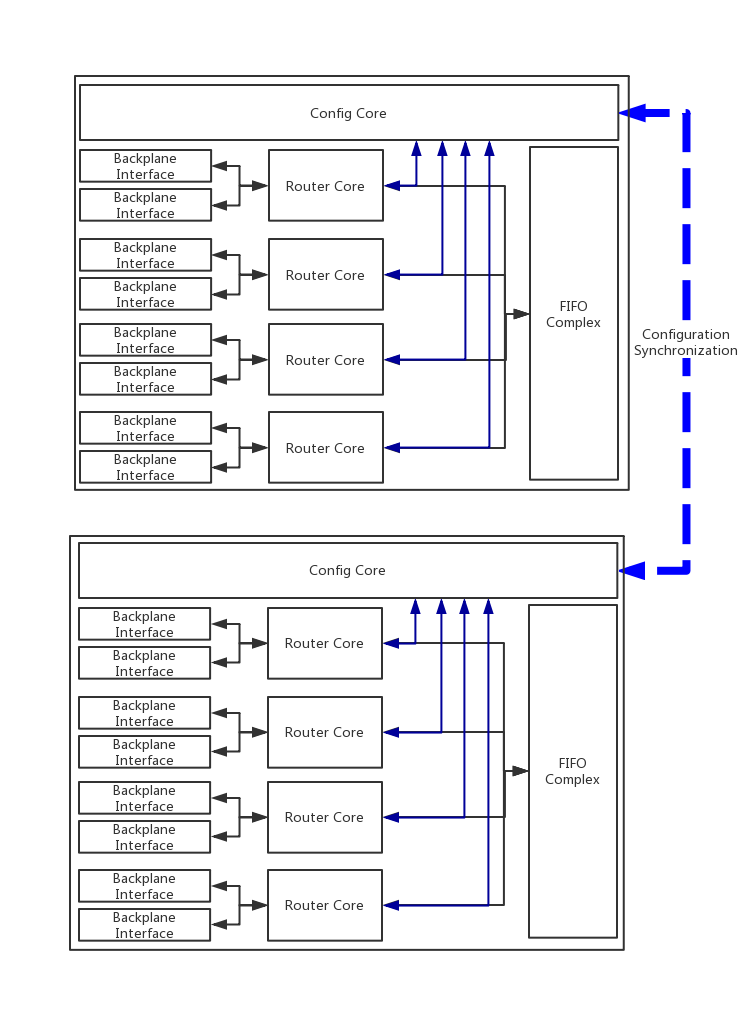
\includegraphics[width=0.7\textwidth]{img/DR00001_SpaceWire_2.png}
 \caption{Data Router Structure}
\end{center}
\end{figure}
\clearpage
\section{CAN + SpaceWire}
\subparagraph{Command Bus}CAN
\subparagraph{Data Bus}SpaceWire\\\\
In this plan, the command bus is using CAN. It provide prioritize data transmission for small amount data transmission. Up to 500kbps bandwidth provide enough bandwidth for command data transmission. The data bus is using the SpaceWire which provide enough bandwidth for high speed data transmission. It also include timestamp feature that will help for the future sensor fusion. The whole system is build base on two router, one is the main router that will use for the major data transmission and the other is backup router which can take over when the main router fail.
\begin{figure}[htp]
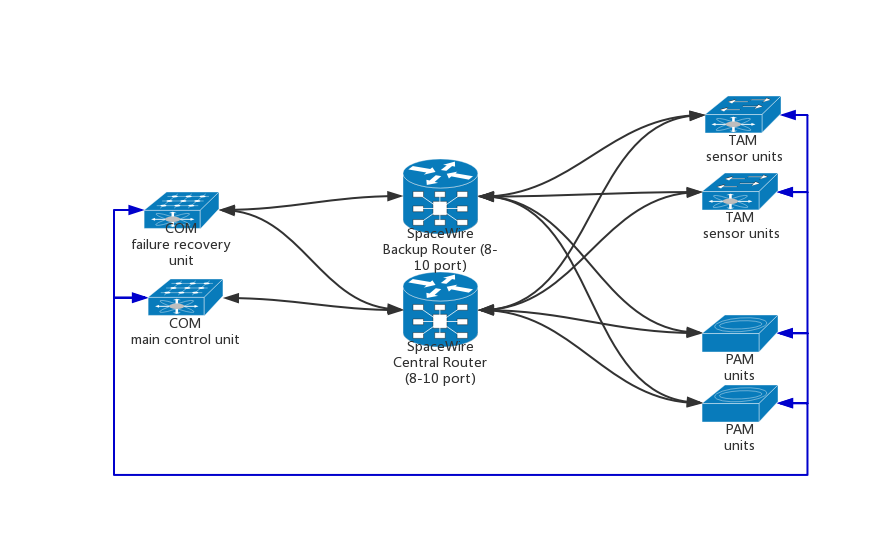
\includegraphics[width=\textwidth]{img/DR00001_SpaceWire_1.png}
 \caption{Recommand Design A}	
\end{figure}
\clearpage
\section{CAN + RapidIO}
\subparagraph{Command Bus}CAN
\subparagraph{Data Bus}RapidIO\\\\
In this plan, CAN bus still is the main command bus due to its prioritize data transmission. In the data bus, RapidIO each lane can carry 10 times data rate compare with the SpaceWire. It can handle most future advance mission without any hardware upgrade. Some company also providing ASIC for rapidIO bus router.
\begin{figure}[htp]
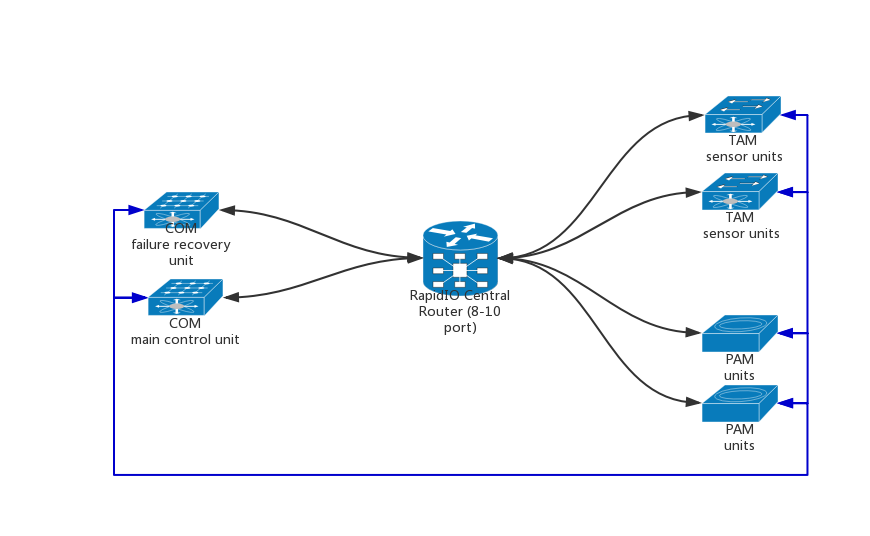
\includegraphics[width=\textwidth]{img/DR00001_RapidIO.png}
 \caption{Recommand Design B}	
\end{figure}
\newpage
%\chapter{OA-II BUS Software Structure}
%\newpage
%end of document
%**********************************************************************
\end{document}